\documentclass[dvipdfmx,uplatex]{jsarticle}

%% Packages
\usepackage{graphicx,color,hyperref}
\usepackage{algorithm}
\usepackage{algorithmic}
\usepackage{url}
\usepackage{lscape}
\usepackage{mathtools}
\usepackage{here}
\usepackage{amsmath,amssymb,amsfonts}
\usepackage{amsthm}
\usepackage{tikz}
\usepackage{tcolorbox}
\usepackage{pxjahyper}

%% Theorem Styles
\newtheorem{theorem}{定理}
\newtheorem{proposition}{命題}
\newtheorem{cor}{系}
\newtheorem{definition}{定義}
\newtheorem{problem}{問題}
\theoremstyle{remark}
\newtheorem{remark}{注意}
\newtheorem{requirement}{条件}

%% Environment (Colorful Box)
\newenvironment{simplebox}{
    \begin{tcolorbox}[
        fonttitle=\bfseries,
    ]
}{
    \end{tcolorbox}
}

\newenvironment{method}[1]{
    \begin{tcolorbox}[
        colframe=green!50!black,
        colback=green!50!black!10!white,
        colbacktitle=green!50!black!40!white,
        coltitle=black,
        fonttitle=\bfseries,
        title={#1}
    ]
}{
    \end{tcolorbox}
}

\newenvironment{experiment}[1]{
    \begin{tcolorbox}[
        colframe=violet,
        colback=violet!10!white,
        colbacktitle=violet!40!white,
        coltitle=black,
        fonttitle=\bfseries,
        title={#1}
    ]
}{
    \end{tcolorbox}
}

\newenvironment{kansou}{
    \begin{tcolorbox}[
        colframe=brown,
        colback=brown!10!white,
        colbacktitle=brown!40!white,
        coltitle=black,fonttitle=\bfseries
    ]
}{
    \end{tcolorbox}
}

%% Title
\title{Text-to-SQL Empowered by Large Language Models: A
Benchmark Evaluation}
\author{\empty}
\date{\empty}

%% Document body
\begin{document}
\maketitle

\begin{itemize}
    \item Link: \url{https://dl.acm.org/doi/10.14778/3641204.3641221}
    \item Conference: VLDB2024
    \item Citation: \cite{text2sql_benchmark}
    \item Arxiv: \url{https://arxiv.org/abs/2308.15363}
\end{itemize}
%% https://gemini.google.com/app/78f907303f22105a


\section{概要}
\begin{simplebox}
\begin{itemize}
    \item Text-to-SQLは、自然言語で書かれた質問をSQLクエリに変換する技術である。
    \item 近年、LLMの発展により、Text-to-SQLの精度が向上している。
    \item 本研究では、Text-to-SQLの性能を評価するためのベンチマークを提案し、様々なLLMを用いた実験を行った。
    \item 提案したText-to-SQLの手法DAIL-SQLが従来の手法よりも高い精度を達成した。
\end{itemize}
\end{simplebox}

%% Text-to-SQLは、自然言語で書かれた質問をSQLクエリに変換する技術である。
%% 近年、LLMの発展により、Text-to-SQLの精度が向上している。
%% 本研究では、Text-to-SQLの性能を評価するためのベンチマークを提案し、様々なLLMを用いた実験を行った。

% \section{背景}
% \begin{simplebox}
% \begin{itemize}
%     \item 自然言語での質問と関連する情報を表現することをQuestion Representation(質問表現)とよぶ。
% \end{itemize}
% \end{simplebox}

% 自然言語での質問と関連する情報を表現するプロセスのことを質問表現(Question Representation)とよぶ。
% インコンテキストラーニング: プロンプト学習。
% 教師ありファインチューニングでその性能をより向上させられることが知られている。

\section{手法}
\begin{method}{Question Representation (質問表現)}
\begin{itemize}
    \item このプロセスは今聞きたい質問$q$に対して, 期待する応答が得られるようなゼロショットのプロンプトを作ることを目的とする.
    \item 5つの主要な方法がある.
    \begin{itemize}
        \item Basic Prompt (BS${}_p$): テーブルスキーマと質問のみ
        \item Text Representation Prompt (TR${}_p$): テーブルスキーマと質問を自然言語で表現する.
        \item OpenAI Demonstration Prompt (OD${}_p$): TR${}_p$に加えて、自然言語で書かれている部分は行頭に$\#$をつける.
        \item Code Representation Prompt (CR${}_p$): テーブルスキーマと質問をコードのように表現する.
        \item Alpaca SFT Prompt (AS${}_p$): プロンプト+テーブルスキーマ+質問を自然言語で与える.
    \end{itemize}
    \item これらの手法はこれまで異なるLLMやデータセットで評価されてきたため、きちんとした比較がされてこなかった。
\end{itemize}
\end{method}

\begin{method}{In-Context Learning}
\begin{itemize}
    \item 「Zero-shotのプロンプト+例となるようなSQLクエリ」を与えることで、LLMが自然言語の質問に対してSQLクエリを生成するように学習させる手法をここでは考える.
    \item このSQLクエリの1. 選び方, 2. 作り方を変化させる
    \item 選び方
    \begin{itemize}
        \item Random: 候補から$k$個ランダムに選ぶ.
        \item Question Similarity Selection (QTS${}_S$): 質問と類似した質問を言語モデルによるベクトル化とベクトル検索を用いて選ぶ.
        \item Masked Question Similarity Selection (MQS${}_S$): テーブル名、列名などドメイン特有の情報をマスクした状態で質問をベクトル化して類似したベクトルを選ぶ.
        \item Query Similarity Selection (QRS${}_S$): 一度ほかの言語モデルでSQLクエリを生成し、それに近いSQLクエリを選ぶ.
    \end{itemize}
    \item 作り方
    \begin{itemize}
        \item Full-information Organization (FI${}_O$): 質問と同じフォーマットで、クエリ例を与える.
        \item SQL-Only Organization (SO${}_O$): SQLクエリのみを表示する.
    \end{itemize}
    \item 上の手法を組み合わせてDAIL-SQLという手法を提案する.
    \item DAIL Selection 
    \begin{itemize}
        \item MSQ${}_S$, QRS${}_S$をいずれもつかい、質問に対して類似したSQLクエリを$k$個選ぶ.
    \end{itemize}
    \item DAIL Organization
    \begin{itemize}
        \item トークン効率と精度を考慮してFI${}_O$とSO${}_O$を組み合わせる.
        \item 具体的には, 質問と対応するSQLクエリのペアを与えるのみで, テーブルスキーマを与えない.
    \end{itemize}
\end{itemize}
\end{method}

\begin{method}{Supervised Fine-tuning}
\begin{itemize}
    \item 上の章で準備したクエリとその期待する応答を用いて、LLMをファインチューニングする.
    \item これは今まで検討されていなかったが、Text-to-SQLタスクにおける, LLMの性能を向上させる可能性がある.
\end{itemize}
\end{method}

\section{実験結果}
\begin{experiment}{実験手法}
\begin{itemize}
    \item Text-to-SQLのさまざまな手法を比較するために様々なLLM, プロンプトなどの手法を用いて実験を行う.
    \item データセット
    \begin{itemize}
        \item Spider: 200以上のデータベースに対する自然言語での質問と対応するSQLクエリとのペアを保持するデータセット.
        \item Spider-Realistic: Spiderと同じフォーマットでSpiderの質問を変更し、より難しい質問を生成したデータセット.
    \end{itemize}
    \item 評価指標
    \begin{itemize}
        \item Exact-set-match accuracy (EM): 予測されたSQLクエリとそれに対応する正解の間のSQLキーワードの一致度を測定する.
        \item Execution accuracy (EX): 予測されたSQLクエリの実行結果と正解のSQLクエリの実行結果の一致度を判定する.
    \end{itemize}
    \item LLM: すべての実験で同じ最大コンテキスト長を利用する.
\end{itemize}
\end{experiment}

\begin{experiment}{実験結果}
\begin{itemize}
    \item Question Representation: 手法のところで紹介された質問表現をゼロショットで評価する.
    \begin{itemize}
        \item 図\ref{fig:question-representation}に示すように、OD${}_p$がどのLLMを用いた場合でも比較的高い精度を達成した.
        \item GPT-4はBS${}_p$のときにもっとも高い精度を達成しており、強力なLLMはQuestion Representationの複雑な表現を必要としない可能性があることが分かった.
    \end{itemize}
    \item In-Context Learning
    \begin{itemize}
        \item 図\ref{fig:in-context-learning}にあるようにDAIL${}_S$が高い性能を示している. GPT-4でDAIL${}_S$を用いた場合、SpiderデータセットでのEMは$71.9\%$, EXは$82.4\%$を達成し, これがもっともよい結果.
        \item またこの図から、クエリ類似度と質問類似度が高くなればなるほど、精度が高くなることが分かる.
        \item Organizationの方法についてはSO${}_O <$DAIL${}_O <$ FI${}_O$の順に精度が高くなることが分かる.
    \end{itemize} 
    \item Supervised Fine-tuning
    \begin{itemize}
        \item オープンソースLLMを用いて, Text-to-SQLタスクに対してファインチューニングする.
        \item 図\ref{fig:fine-tuning}に示すようにファインチューニングしたモデルでのZero-shotプロンプトを用いた場合の精度を示す.
        \item CR${}_p$が良い精度を達成する.
        \item アラインメントがよい結果をもたらすことがわかる.
    \end{itemize}
    \item トークン効率
    \begin{itemize}
        \item DAIL${}_O$はSO${}_O$と同じくらいのトークン効率で, FI${}_O$と同じくらいの精度を達成することがわかる.
    \end{itemize}
\end{itemize}
\end{experiment}

\begin{figure}
    \centering
    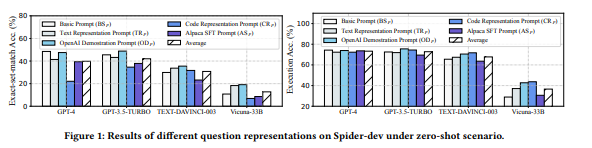
\includegraphics[width=0.8\textwidth]{img/text2sql-with-llm/question-representation.png}
    \caption{Question Representationに関する結果}
    \label{fig:question-representation}
\end{figure}

\begin{figure}
    \centering
    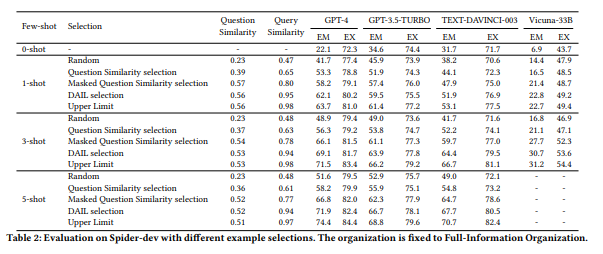
\includegraphics[width=0.8\textwidth]{img/text2sql-with-llm/icl.png}
    \caption{In-Context Learningに関する結果}
    \label{fig:in-context-learning}
\end{figure}

\begin{figure}
    \centering
    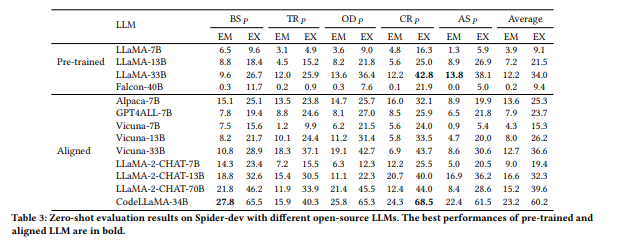
\includegraphics[width=0.8\textwidth]{img/text2sql-with-llm/fine-tuning.png}
    \caption{Fine tuningに関する結果}
    \label{fig:fine-tuning}
\end{figure}

\section{感想}
\begin{kansou}
\begin{itemize}
  \item Text-to-SQLのタスクってかなり難しそうだけど、LLMによってできなくはないくらいにはなるのだなと思った.
  \item LLMがコストがとても大きいクエリを生成する可能性や、セキュリティなどのことを考えると実際に使うには、うまく使わないといけなさそうだなと思った.
\end{itemize}
\end{kansou}

\bibliographystyle{jplain}
\bibliography{template.bib}

\end{document}